\documentclass[10pt,bahasa]{article}
\usepackage[a4paper]{geometry}
\geometry{verbose,tmargin=1.5cm,bmargin=1.5cm,lmargin=1.5cm,rmargin=1.5cm}
\usepackage{amsmath}
    
\setlength{\parindent}{0cm}
  
\usepackage{float}
\usepackage{graphicx}
\usepackage{enumitem}
\usepackage{hyperref}
\usepackage{url}
\usepackage{xcolor}
\usepackage{babel}

\usepackage{minted}
\newminted{scilab}{breaklines}

\definecolor{mintedbg}{rgb}{0.95,0.95,0.95}
\usepackage{mdframed}

\BeforeBeginEnvironment{minted}{\begin{mdframed}[backgroundcolor=mintedbg]}
\AfterEndEnvironment{minted}{\end{mdframed}}

\begin{document}

\title{Tugas Besar TF2202}
\date{}
\maketitle

Selesaikan soal-soal berikut ini dengan menggunakan Scilab.

%=====================================================
\section{Perbandingan akurasi beberapa metode untuk ODE}
%=====================================================

Carilah solusi numerik dari persamaan diferensial berikut
\begin{equation}
y''(t) + y(t) = 0
\end{equation}
dengan syarat awal
\begin{equation}
y(0) = 0, \hspace{0.5cm} y'(0) = 1
\end{equation}
pada interval $0 \leq t \leq 10$.

Bandingkan solusi yang diperoleh dengan solusi analitik:
\begin{equation}
y(t) = \sin(t)
\end{equation}

Gunakan menggunakan metode-metode berikut ini untuk mencari solusi numeriknya.
\begin{itemize}
\item Euler
\item Euler dengan prediktor-korektor (Runge-Kutta orde-2)
\item Runge-Kutta orde-4
\end{itemize}

Dari solusi numerik yang didapatkan, buatlah (1) plot antara $y$ dan $y'$
dan (2) plot antara $t$ dan $y$.

\subsection*{Solusi}

Metode Euler file (file: \texttt{ode\_euler.sce})

\begin{scilabcode}
function [t,y] = ode_euler(f,tspan,y0,N)
    
  if (~exists("N", "local")) | (N <= 0)
    N = 100
  end
    
  if ~exists("tspan","local")
    y0 = 0
  end
    
  h = (tspan(2) - tspan(1))/N
  t = tspan(1) + [0:N]'*h
    
  // check y0, transpose if needed
  if size(y0,1) ~= 1
    if size(y0,2) > 1
      y0 = y0'
    end
  end
  
  Ndim = size(y0,2)
  y = zeros(N+1,Ndim)
    
  // initial value
  y(1,:) = y0
  
  // Euler's algorithm here
  for k = 1:N
    y(k+1,:) = y(k,:) + h*f(t(k),y(k,:))
  end
  
endfunction  
\end{scilabcode}


Metode Euler dengan prediktor-korektor: (file: \texttt{ode\_euler\_PC.sce})

\begin{scilabcode}
function [t,y] = ode_euler_PC(f,tspan,y0,N)
  
  if (~exists("N", "local")) | (N <= 0)
    N = 100
  end
  
  if ~exists("tspan","local")
    y0 = 0
  end
  
  h = (tspan(2) - tspan(1))/N
  t = tspan(1) + [0:N]'*h
  
  // check y0, transpose if needed
  if size(y0,1) ~= 1
    if size(y0,2) > 1
      y0 = y0'
    end
  end

  Ndim = size(y0,2)
  y = zeros(N+1,Ndim)
  
  // initial value
  y(1,:) = y0

  for k = 1:N
    yk1 = y(k,:) + h*f( t(k), y(k,:) )
    y(k+1,:) = y(k,:) + 0.5*h*( f(t(k),y(k,:)) + f(t(k)+h,yk1) )
  end

endfunction
\end{scilabcode}

Metode Runge-Kutta orde 4 (file: \texttt{ode\_RK4.sce})

\begin{scilabcode}
function [t,y] = ode_RK4(f,tspan,y0,N)
  //
  if (~exists("N", "local")) | (N <= 0)
    N = 100
  end
  //
  if ~exists("tspan","local")
    y0 = 0
  end
  // check y0, transpose if needed
  if size(y0,1) ~= 1
    if size(y0,2) > 1
      y0 = y0'
    end
  end
  //
  Ndim = size(y0,2)
  y = zeros(N+1,Ndim)
  //
  y(1,:) = y0
  h = (tspan(2) - tspan(1))/N
  t = tspan(1) + [0:N]'*h
  h2 = h/2
  // Runge-Kutta 4th-order algorithm here
  for k=1:N
    f1 = h*f(t(k),y(k,:))
    f2 = h*f(t(k)+h2,y(k,:)+f1/2)
    f3 = h*f(t(k)+h2,y(k,:)+f2/2)
    f4 = h*f(t(k)+h,y(k,:)+f3)
    y(k+1,:) = y(k,:) + (f1 + 2*(f2+f3) + f4)/6
  end
endfunction
\end{scilabcode}

Contoh hasil solusi:

\begin{scilabcode}
exec("ode_euler.sce",-1)
exec("ode_euler_PC.sce",-1)
exec("ode_RK4.sce",-1)

// definisi ODE
function f = dy(t,y)
  f(1) =  y(2)
  f(2) = -y(1)
  f = f'
endfunction
  
tspan = [0 10]
y0 = [0 1]
  
method = "RK4" // pilih metode
  
h = 0.05
N = (tspan(2) - tspan(1))/h
  
if method == "RK4"
  [t,y] = ode_RK4(dy,tspan,y0,N)
elseif method == "euler"
  [t,y] = ode_euler(dy,tspan,y0,N)
elseif method == "euler_PC"
  [t,y] = ode_euler_PC(dy,tspan,y0,N)  
else
  error("method is unknown")
end
  
clf()
plot( y(:,1), y(:,2), 'b' )
// xmin, ymin, xmax, ymax
xlabel('$y_1$')
ylabel('$y_2$')
if method == "euler"
  square(-15,-15,15,15)
  xs2pdf( gcf(), "images/soal_01_ode_euler_y1_y2.pdf" )
elseif method == "euler_PC"
  square(-1.5,-1.5,1.5,1.5)
  xs2pdf( gcf(), "images/soal_01_ode_euler_PC_y1_y2.pdf" )  
elseif method == "RK4"
  square(-1.5,-1.5,1.5,1.5)
  xs2pdf( gcf(), "images/soal_01_ode_RK4_y1_y2.pdf" )
end
  
clf()
plot( t, y(:,1), 'b')
xlabel('$t$')
ylabel('$y_1$')
if method == "euler"
  xs2pdf( gcf(), "images/soal_01_ode_euler_t_y1.pdf")
elseif method == "euler_PC"
  set(gca(),"data_bounds",[0,100,-1.2,1.2])
  xs2pdf( gcf(), "images/soal_01_ode_euler_PC_t_y1.pdf")  
elseif method == "RK4"
  set(gca(),"data_bounds",[0,100,-1.2,1.2])  
  xs2pdf( gcf(), "images/soal_01_ode_RK4_t_y1.pdf")
end
\end{scilabcode}

Hasil visualisasi solusi

\begin{figure}[H]
{\centering
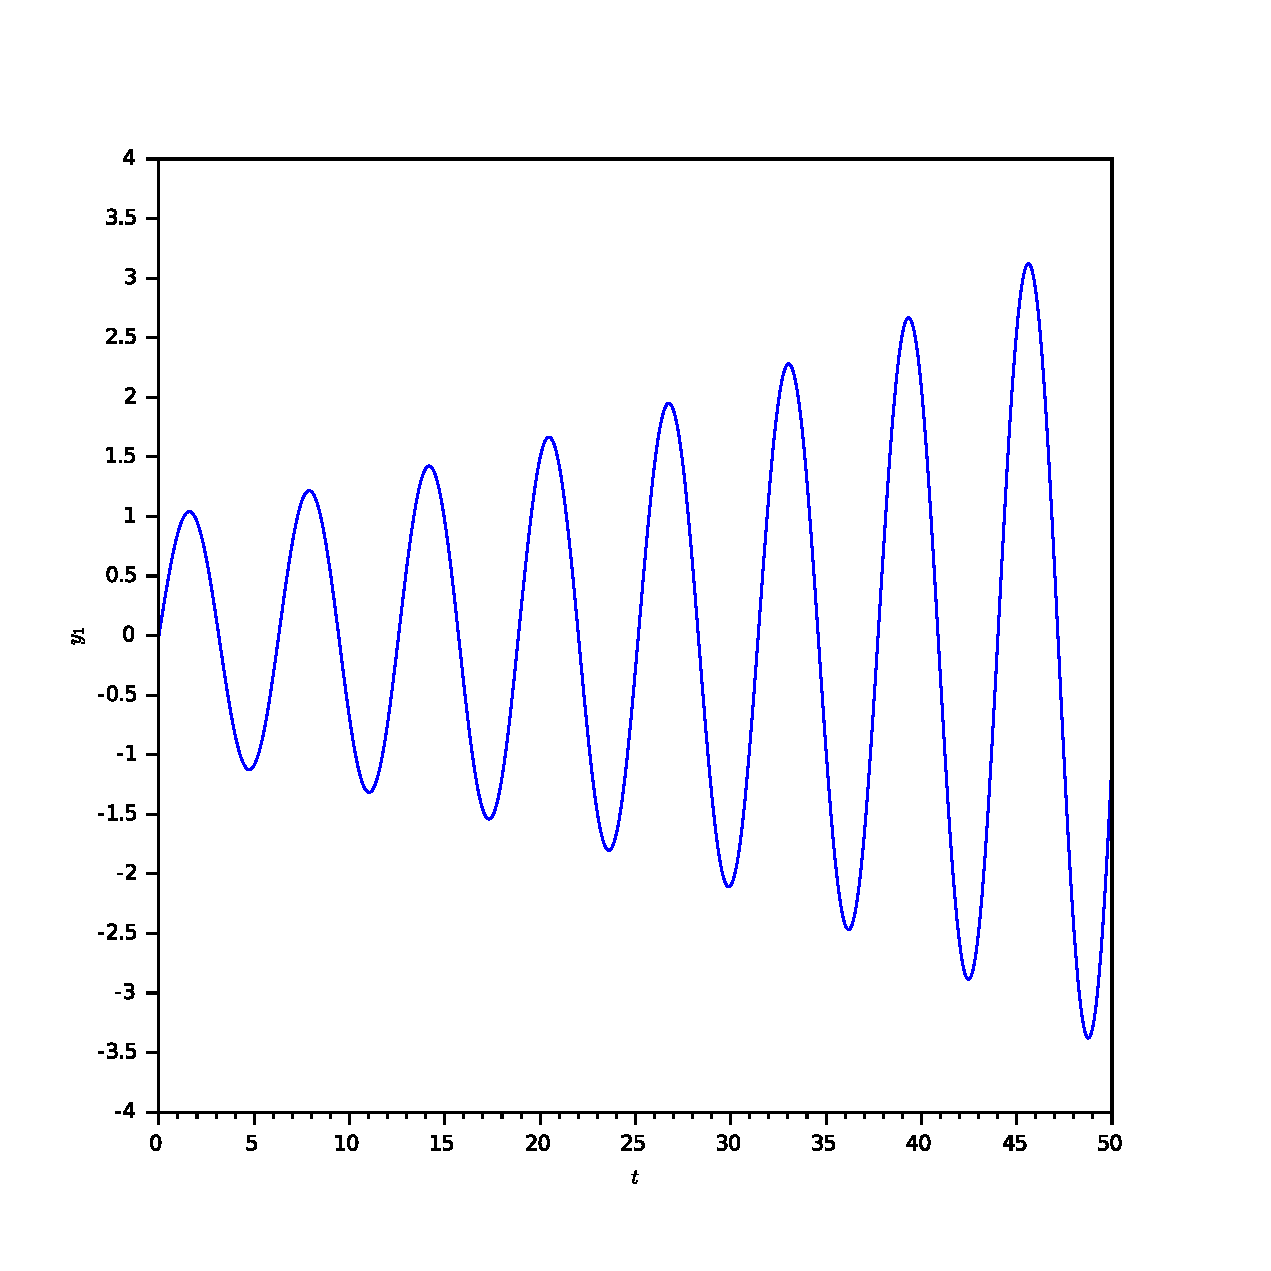
\includegraphics[width=0.3\textwidth]{images/soal_01_ode_euler_t_y1.pdf}
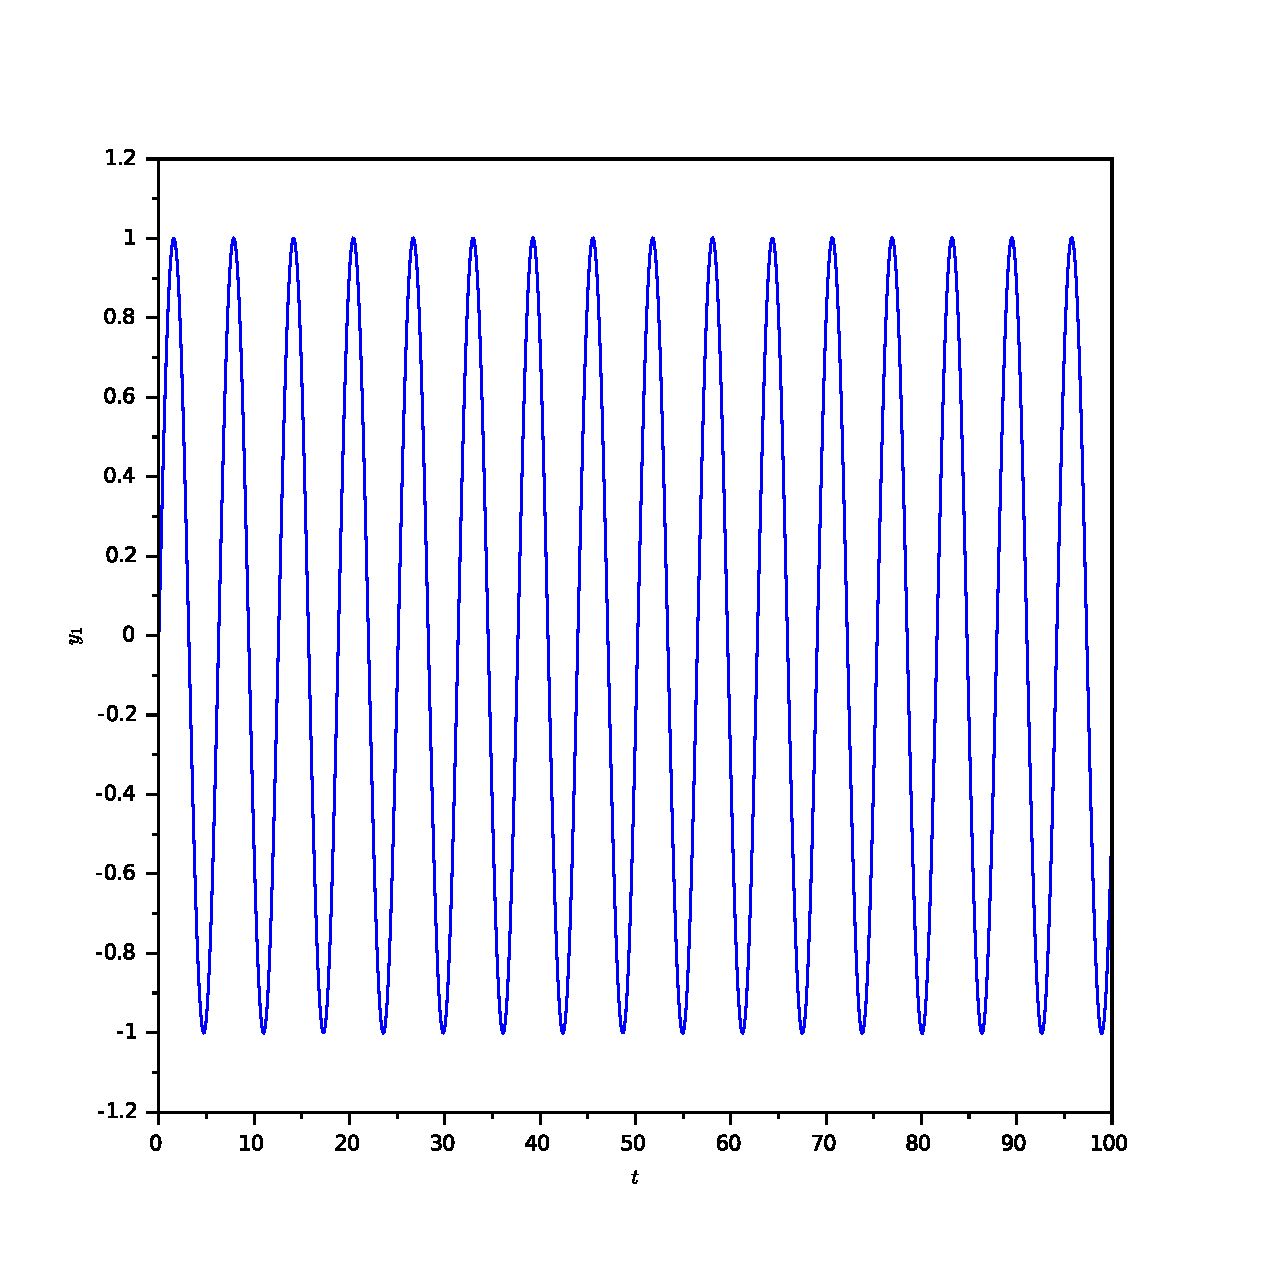
\includegraphics[width=0.3\textwidth]{images/soal_01_ode_euler_PC_t_y1.pdf}
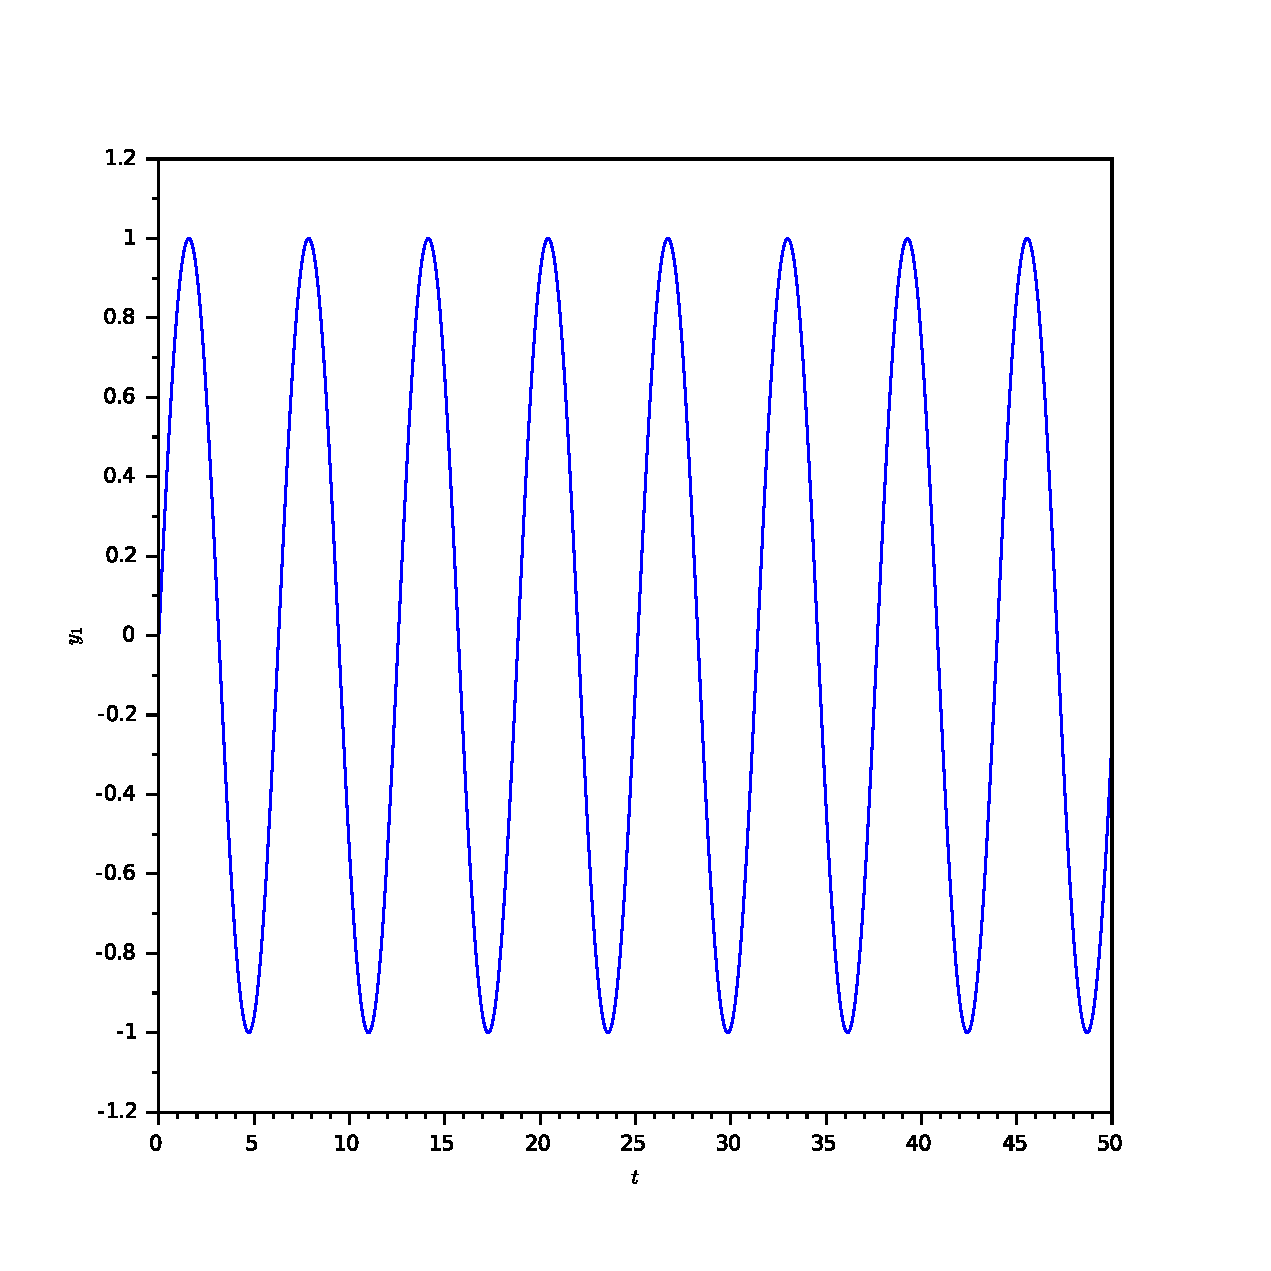
\includegraphics[width=0.3\textwidth]{images/soal_01_ode_RK4_t_y1.pdf}
\par}
\caption{Hasil solusi numerik $x$ vs $y_1$, berturut-turut dari kiri ke kanan:
Euler, Euler dengan prediktor-korektor dan Runge-Kutta orde 4}
\end{figure}

%=================================
\section{Gerakan pendulum}
%=================================

Gerak suatu pendulum dapat dinyatakan dengan persamaan diferensial:
\begin{equation}
\theta''(t) = -\frac{g}{L}\sin(\theta(t)) - k\theta'(t)
\end{equation}
dengan syarat awal
\begin{equation}
\theta(0) = \theta_0, \hspace{0.5cm} \theta'(0) = 0
\end{equation}

\begin{figure}[H]
\centering
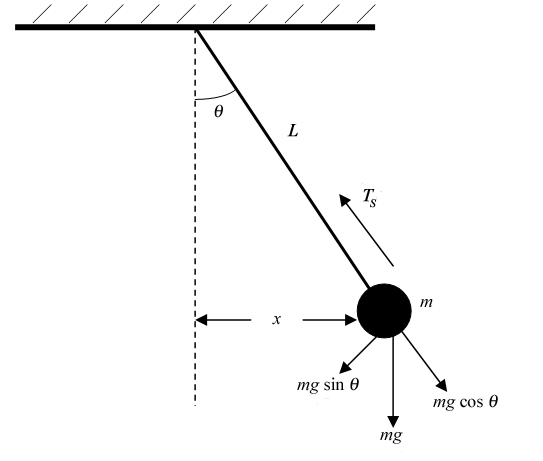
\includegraphics[scale=0.4]{images/pendulum.png}
\par
\caption{Pendulum sederhana}
\end{figure}

Dalam persamaan tersebut $\theta$ menyatakan simpangan pendulum,
$\theta_0$ menyatakan simpangan awal pendulum,
$g$ menyatakan percepatan gravitasi, $L$ menyatakan panjang benang pendulum,
dan $k\theta'$ menyatakan suku redaman (gesekan) yang berbanding lurus
dengan kecepatan $\theta'$ ($k$ adalah bilangan positif).

\begin{enumerate}[label=(\alph*)]
\item Cari solusi $\theta(t)$ untuk kasus $k=0$ untuk simpangan awal $\theta_0 = 0.1, \pi/5$
dan 3.0.
\item Masih untuk kasus $k=0$, tentukan periode osilasi $T$ sebagai
fungsi dari simpangan awal $u_0$.
\item Carilah solusi $u(t)$ untuk kasus $k = 0.1, 0.3, 0.5$ dan 0.8 untuk
simpangan awal yang sama.
\end{enumerate}


%========================================================
\section{Persamaan Schrodinger (metode shooting)}
%========================================================

Persamaan Schrodinger independen-waktu pada 1 dimensi
dapat dinyatakan sebagai berikut.
\begin{equation}
-\frac{\hbar^2}{2m}\frac{\mathrm{d}\psi}{\mathrm{d}x^2}
+ V(x)\psi(x) = E\psi(x)
\label{eq:sch1d}
\end{equation}
Dengan menggunakan unit atomik, kita dapat mengambil $\hbar = 1$
dan $m = 1$, dan persamaan \eqref{eq:sch1d} dapat ditulis menjadi:
\begin{equation}
\psi'' = 2\left[ V(x) - E \right]\psi
\label{eq:sch1d_2}
\end{equation}
Untuk solusi keadaan terikat (bound states), nilai $E$ hanya dapat memiliki
nilai yang diskrit. Selain itu, untuk bound states
fungsi gelombang dibatasi dengan syarat
\begin{equation}
\lim_{x\rightarrow\infty} \psi(x) = 0,\hspace{0.5cm}\lim_{x\rightarrow-\infty} \psi(x) = 0
\end{equation}
Selain itu, fungsi gelombang biasanya juga dinyatakan dalam bentuk ternormalisasi:
\begin{equation}
\int_{-\infty}^{\infty} \psi^{*}(x) \psi(x)\,\mathrm{d}x = 1
\end{equation}

Untuk potensial yang simetrik terhadap $x=0$, secara matematis dapat ditulis
$V(-x) = V(x)$. Contoh potential simetrik yang akan dibahas adalah potensial harmonik
\begin{equation}
V(x) = \frac{1}{2}x^2
\end{equation}
Dengan demikian, kita bisa mendapatkan solusi pada $(-\infty,\infty)$ hanya dengan
solusi pada $(0,\infty)$.
Ingat lagi dari kuliah mekanika kuantum bahwa,
untuk potensial harmonik, nilai $E$ yang diperbolehkan adalah:
\begin{equation}
E = \frac{(n + 1)}{2}, \hspace{0.5cm} n = 0,1,2,\ldots
\end{equation}
Kita dapat mengelompokkan solusi ini menjadi dua kelompok:
\begin{itemize}
\item solusi ganjil ($n = 1, 3, 5, \ldots$), dengan fungsi gelombang
$\psi(x) = -\psi(-x)$
\item solusi genap ($n = 0, 2, 4, \ldots$), dengan fungsi gelombang
$\psi(x) = \psi(-x)$
\end{itemize}

Persamaan \eqref{eq:sch1d_2} dapat diselesaikan dengan
menggunakan metode standard seperti Runge-Kutta
orde-4. Metode lain yang sering digunakan adalah metode Numerov. Metode ini biasa
digunakan untuk menyelesaikan persamaan diferensial orde dua tanpa suku dengan turunan
pertama, seperti pada persamaan \eqref{eq:sch1d_2}.
Metode ini dapat dituliskan dalam bentuk:
\begin{align}
u_{m} & = 1 - \dfrac{1}{6}h^2 \left[ V(x_m) - E \right] \\
\psi_{m+1} & = \dfrac{\left(12 - 10u_{m}\right)\psi_{m} - u_{m-1}\psi_{m-1}}{u_{m+1}}
\end{align}

Untuk mengaplikasikan metode shooting, persamaan nilai batas harus dikonversi menjadi
permasalahan syarat awal:
\begin{align}
\psi(0) & = \psi_{0},\hspace{0.5cm} \psi'(0) = 0,\hspace{0.5cm} n = 0,2,4,\ldots \\
\psi(0) & = 0,\hspace{0.5cm} \psi'(0) = \psi'_{0},\hspace{0.5cm} n = 1,3,5,\ldots
\end{align}
Nilai dari $\psi_0$ dan $\psi'_0$ dapat dipilih dengan nilai sembarang bukan nol.
Untuk soal ini kita akan ambil $\psi_0 = 1$ dan $\psi'_0 = 1$.

\begin{enumerate}[label=(\alph*)]
\item Buatlah program untuk menghitung solusi numerik dari persamaan \ref{eq:sch1d_2}
dengan menggunakan metode Numerov. Perhatikan bahwa untuk mendapatkan nilai $\psi_{m+1}$ kita memerlukan dua nilai
sebelumnya, yaitu $\psi_{m}$ dan $\psi_{m-1}$, sedangkan dari deskripsi masalah kita
biasanya hanya memiliki informasi nilai awal $\psi_{0}$ dan $\psi'_{0}$.
Untuk mencari nilai $\psi_{1}$ kita dapat menggunakan metode Euler-Cromer:
\begin{equation}
\psi_{1} = \psi_{0} + \psi'_{0}\Delta x + 2(V(x_{0}) - E)(\Delta x)^2
\end{equation}
Gunakan nilai solusi analitik $E = 0.5$ dan disekitarnya misalnya $E = 0.499$ dan $0.501$
serta bandingkan hasilnya numerik dari $\psi$ yang didapatkan dengan
$\psi$ eksak, yaitu $\psi = \exp(-x^2/2)$.
Anda dapat mengaproksimasi solusi pada selang $0 \leq x < \infty$
dengan solusi selang $0 < x < 5$, misalnya dengan asumsi bahwa fungsi gelombang
eksak telah memiliki nilai nol pada $x = 5$.
Gunakan juga syarat awal yang sesuai untuk $E = 0.5$ (solusi genap), yaitu
$\psi_{0} = 1$ dan $\psi'_{0} = 0$.
%
\item Gunakan metode shooting dengan cara memvariasikan nilai $E$ untuk mencari
nilai $E$ yang mungkin dalam rentang $0 \leq E \leq 15$. Gunakan syarat awal
yang sesuai untuk solusi ganjil dan genap.
\end{enumerate}


%====================================================
\section{Persamaan Schrodinger (nilai eigen)}
%====================================================

Metode alternatif
yang dapat digunakan untuk menyelesaikan persamaan
Schrodinger independen-waktu adalah dengan menyelesaikan
persamaan eigenvalue
\begin{align}
\left[-\frac{\mathrm{d}^2}{\mathrm{d}x^2} + V(x)\right]\psi(x) & = E\psi(x) \\
\hat{H}\psi(x) & = E \psi(x)
\end{align}
Nilai-nilai $E$ yang mungkin dapat dicari dengan cara menghitung
nilai eigen dari matriks Hamiltonian 
\begin{equation}
H_{ij} = K_{ij} + V_{ij}
\end{equation}
Dengan $K_{ij}$ dan $V_{ij}$ adalah representasi matriks dari operator
kinetik dan potensial.
Fungsi eigen terkait adalah fungsi gelombang solusi dari
persamaan \eqref{eq:sch1d_2}.

Suatu selang $-L < x < L$ dengan $L$ suatu bilangan positif
dibagi-bagi kedalam $N-1$ partisi dengan jumlah total titik $N$,
yaitu $x_{i}$, $i = 1, 2, \ldots, N$.
Potensial $V(x)$ dapat dihitung pada $x_{i}$ sehingga
kita peroleh representasi diskrit dari potensial:
$V_{i} = V_(x_{i})$.

Matriks $V_{ij}$ adalah matriks diagonal yang elemen diagonalnya adalah
nilai dari $V(x)$ pada titik $x_{i}$.

Matriks $K_{ij}$ dapat
dapat diaproksimasi dengan cara mengaproksimasi operator $\mathrm{d}^2/\mathrm{d}x^2$
dengan menggunakan beda hingga.

\begin{enumerate}[label=(\alph*)]
\item Gunakan beda hingga sentral 3 titik untuk mengaproksimasi matriks $K_{ij}$
\item Hitung matriks Hamiltonian dan selesaikan persamaan eigen $H\psi = E\psi$. Anda dapat
menggunakan perintah \texttt{[psi,D] = spec(H); E = diag(D)} pada Scilab.
Bandingkan hasil yang Anda peroleh dengan solusi analitik.
\item Ulangi (a) dan (b) dengan menggunakan beda hingga sentral 5, 7, dan 9 titik.
Bandingkan hasilnya dengan menggunakan $\Delta x$ yang sama.
\end{enumerate}


\section{Persamaan Poisson 2D}

Hitung solusi numerik dari persamaan Laplace:
\begin{equation}
\frac{\partial^2 u(x,y)}{\partial x^2} +
\frac{\partial^2 u(x,y)}{\partial y^2} = \cos(x + y) - \sin(x - y)
\end{equation}
pada domain rektangular $-\pi < x < \pi$, $-\pi < y < \pi$ dengan syarat batas
\begin{equation}
u(\pm\pi,y) = 0, \hspace{0.5cm} u(x,\pm\pi) = 0
\end{equation}
dengan menggunakan metode beda hingga. Gunakan metode Gauss-Seidel untuk
menyelesaikan sistem persamaan linear yang dihasilkan.
Bandingkan solusi numerik yang diperoleh dengan
solusi analitik
\begin{equation}
u(x,y) = \sin(x)\cos(y)
\end{equation}

\begin{figure}[H]
\centering
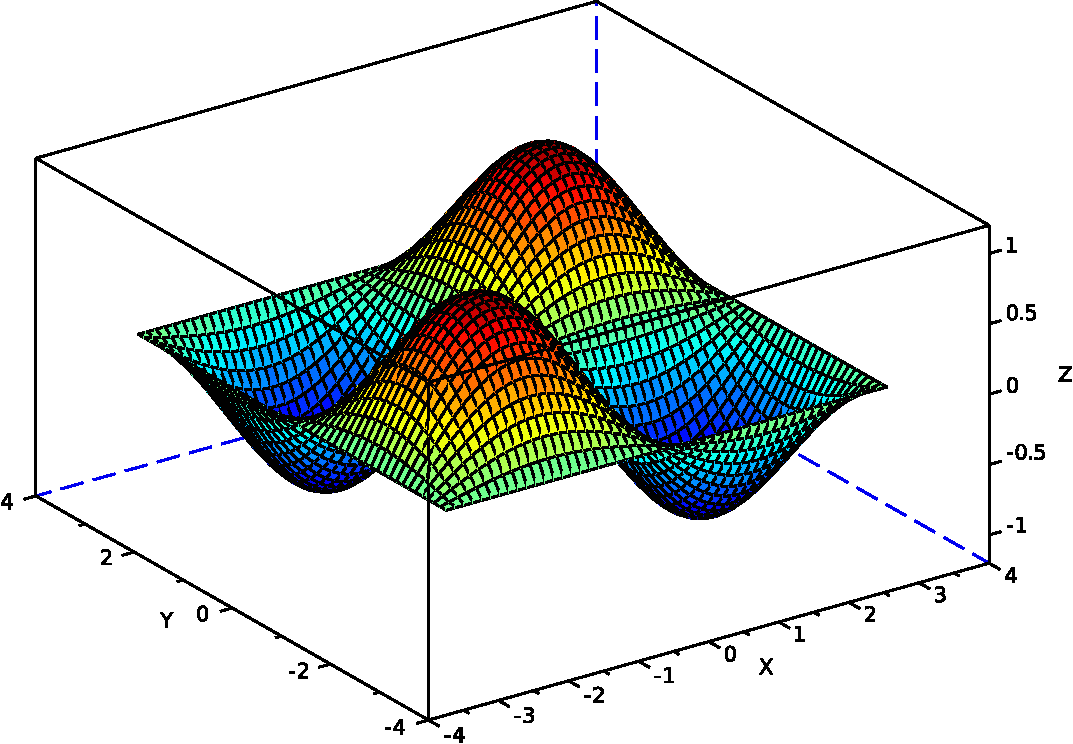
\includegraphics[scale=0.5]{poisson2d.pdf}
\par
\caption{Solusi persamaan Laplace $u(x,y)$}
\end{figure}

\subsection*{Solusi}

Fungsi untuk menyelesaikan persamaan Poisson 2d dengan metode Gauss-Seidel

\begin{scilabcode}
function u = poisson2d(u0, x, y, Nx, Ny, TOL, f)
// Nx, Ny: no of nodes in x and y direction

  MaxIter = 10000 // no. iterative steps

  hx = (x(Nx) - x(1))/(Nx-1)
  kx = 1.0/(hx*hx)

  hy = (y(Ny) - y(1))/(Nx-1)
  ky = 1.0/(hy*hy)

  kxy = 2.0*(kx + ky)

  // Gauss-Seidel algorithm here
  u = u0
  for iter =1:MaxIter
    err = 0.0
    u_old = u
    // loop only for internal nodes
    for j = 2:Ny-1
      for i = 2:Nx-1
        u(i,j) = ( kx*( u(i-1,j) + u(i+1,j) ) + ...
                   ky*( u(i,j-1) + u(i,j+1) ) - f(i,j) ) / kxy
      end
    end
    // calculate error
    err = sum(abs(u - u_old))
    printf("iter = %8d, err = %18.10e\n", iter, err)
    if err < TOL
      printf("Convergence is achieved\n")
      break
    end
  end

endfunction
\end{scilabcode}

Test program:

\begin{scilabcode}
exec("poisson2d.sce",-1)

// RHS of the equation
function u = func(x,y)
  u = cos(x+y) - cos(x-y)
endfunction
  
Nx = 50
Ny = 50
x = linspace(-%pi,%pi,Nx)
y = linspace(-%pi,%pi,Ny)
  
u0 = zeros(Nx,Ny)
// set BC
u0(1,:) = 0.0
u0(:,1) = 0.0
u0(Nx,:) = 0.0
u0(:,Ny) = 0.0

// calculate array for RHS
f = zeros(Nx,Ny)
for j = 1:Ny
  for i = 1:Nx
    f(i,j) = func( x(i), y(j) )
  end
end
  
u = poisson2d(u0, x, y, Nx, Ny, 1e-5, f)
  
surf(x,y,u)
set(gcf(),"color_map",jetcolormap(32))
//colorbar(min(u),max(u))
xs2pdf(gcf(),"poisson2d.pdf")
\end{scilabcode}


\section{Persamaan transfer kalor}

Hitung solusi numerik dari
\begin{equation}
\frac{\partial^2 u(x,t)}{\partial x^2} = \frac{\partial u(x,t)}{\partial t}
\end{equation}
untuk $0 \leq x \leq 1$ dan $0 \leq t \leq 0.1$ dengan syarat awal
\begin{equation}
u(x,0) = \sin(\pi x)
\end{equation}
dan syarat batas
\begin{equation}
u(0,t) = 0,\hspace{0.5cm} u(1,t) = 0
\end{equation}
Gunakan metode Euler eksplisit, Euler implisit dan Crank-Nicolson serta
bandingkan hasilnya.
Buat juga animasi (dalam format GIF) yang menggambarkan perubatan profil
suhu terhadap waktu.

\subsection*{Solusi}

Metode Euler eksplisit:

\begin{scilabcode}
function [u,x,t] = heat_1d_euler_exp(a,xf,T,initialTemp,bx0,bxf,Nx,Nt)

  dx = xf/Nx
  x  = [0:Nx]'*dx
  
  dt = T/Nt
  t  = [0:Nt]*dt
  
  // Set initial condition
  for i = 1:Nx+1
    u(i,1) = initialTemp(x(i))
  end
    
  for it = 1:Nt+1
    u([1 Nx+1],it) = [bx0(t(it)); bxf(t(it))]
  end
    
  r  = a*dt/dx/dx
  r1 = 1 - 2*r
  
  if r > 0.5
    printf("\nheat_1d_euler_exp:\n")
    printf("WARNING: r is larger than 0.5: %f\n", r)
    printf("WARNING: solution is not stable\n\n")
  else
    printf("\nheat_1d_euler:\n")
    printf("r = %f >= 0.5\n", r)
    printf("The solution should be stable\n\n")
  end
  
  for it = 1:Nt
    for i = 2:Nx
      u(i,it+1) = r*( u(i+1,it) + u(i-1,it) ) + r1*u(i,it)
    end
  end
   
endfunction  
\end{scilabcode}

Metode Euler implisit

\begin{scilabcode}
function [u,x,t] = heat_1d_euler_imp(a,xf,T,initialTemp,bx0,bxf,Nx,Nt)

  dx = xf/Nx
  x  = [0:Nx]'*dx
  
  dt = T/Nt
  t  = [0:Nt]*dt
  
  for i = 1:Nx+1
    u(i,1) = initialTemp(x(i))
  end
  
  for it = 1:Nt+1
    u([1 Nx+1],it) = [bx0(t(it)); bxf(t(it))]
  end
  
  r  = a*dt/dx/dx
  r2 = 1 + 2*r
  
  // Build matrix A
  for i = 1:Nx-1
    A(i,i) = r2
    if i > 1
      A(i-1,i) = -r
      A(i,i-1) = -r
    end
  end
  
  // time-stepping, solve linear equation
  for k=2:Nt+1
    b = [r*u(1,k); zeros(Nx-3,1); r*u(Nx+1,k)] + u(2:Nx,k-1);
    u(2:Nx,k) = A\b
  end
  
endfunction  
\end{scilabcode}

Metode Crank-Nicolson

\begin{scilabcode}
function [u,x,t] = heat_1d_CN(a,xf,T,initialTemp,bx0,bxf,Nx,Nt)
  
  dx = xf/Nx
  x  = [0:Nx]'*dx
    
  dt = T/Nt
  t  = [0:Nt]*dt
  
  for i = 1:Nx+1
    u(i,1) = initialTemp(x(i))
  end
  
  for it = 1:Nt+1
    u([1 Nx+1],it) = [bx0(t(it)); bxf(t(it))]
  end
  
  r  = a*dt/dx/dx
  r1 = 2*(1-r)
  r2 = 2*(1+r)
  
  // Build matrix A
  A = zeros(Nx-1,Nx-1)
  for i = 1:Nx-1
    A(i,i) = 2*(1 + r)
    if i > 1
      A(i-1,i) = -r
      A(i,i-1) = -r
    end
  end
  
  // Build matrix B
  B = zeros(Nx-1,Nx-1)
  for i = 1:Nx-1
    B(i,i) = 2*(1 - r)
    if i > 1
      B(i-1,i) = r
      B(i,i-1) = r
    end
  end

  // Time-steping, solve linear equation
  for it = 2:Nt+1
    b = B*u(2:Nx,it-1)
    u(2:Nx,it) = A\b
  end
  
  endfunction  
\end{scilabcode}

Contoh pemanggilan fungsi:

\begin{scilabcode}
exec("to_string.sce",-1)
exec("heat_1d_euler_exp.sce",-1)
exec("heat_1d_euler_imp.sce",-1)
exec("heat_1d_CN.sce",-1)

// initial condition (function of x)
function T = it0(x)
  T = sin(%pi*x)
endfunction

// boundary condition (function of t)
function T = bx0(t)
  T = 0.0
endfunction

function T = bxf(t)
  T = 0.0
endfunction

function T = analytic_solution(x,t)
  T = sin(%pi*x)*exp(-%pi*%pi*t)
endfunction

function plot_to_png(u,x,t,prefix)
  Nt = length(t)-1
  for it = 1:Nt+1
    clf()
    plot(x,u(:,it))
    set(gca(), "data_bounds", [0,1,0,1])
    strt = "t = " + string(t(it))
    xstring(0.8,0.9,strt)
    xs2png(gcf(), prefix + to_string(it) + ".png")
    printf("Done output solution for t = %f\n", t(it))
  end
endfunction

a = 1

xf = 1
Nx = 25

T  = 0.1
Nt = 100

// Explicit Euler
[u1,x,t] = heat_1d_euler_exp( a, xf, T, it0, bx0, bxf, Nx, Nt )
plot_to_png(u1,x,t,"TEMP_exp_")

// Using implicit Euler method
[u2,x,t] = heat_1d_euler_imp( a, xf, T, it0, bx0, bxf, Nx, Nt )
plot_to_png(u2,x,t,"TEMP_imp_")

// Using Crank-Nicholson method
[u3,x,t] = heat_1d_CN( a, xf, T, it0, bx0, bxf, Nx, Nt )
plot_to_png(u3,x,t,"TEMP_CN_")

NxNt = Nx*Nt
u_analytic = analytic_solution(x,t)

//How far from the analytical solution?
err1 = norm((u1-u_analytic))/NxNt
err2 = norm((u2-u_analytic))/NxNt
err3 = norm((u3-u_analytic))/NxNt

printf("err1 = %f\n", err1)
printf("err2 = %f\n", err2)
printf("err3 = %f\n", err3)
\end{scilabcode}


\section{Persamaan gelombang}

Selesaikan PDE berikut dengan menggunakan metode beda hingga.
Buat juga visualisasi solusi berupa animasi dari solusi yang didapatkan.

\begin{enumerate}[label=(\alph*)]
%
\item Hitung solusi numerik persamaan gelombang 1d
\begin{equation}
\frac{\partial^2 u(x,t)}{\partial x^2} = \frac{\partial^2 u(x,t)}{\partial t^2}
\end{equation}
untuk $0 < x < 1$ dan $0 \leq t \leq 1$ dengan syarat awal
\begin{align*}
u(x,0)  & = \sin\left(2\pi x\right) \\
u'(x,0) & = 0
\end{align*}
dan syarat batas:
\begin{equation*}
u(0,t) = 0, \hspace{0.5cm} u(1,t) = 0
\end{equation*}
%
\item Selesaikan persamaan gelombang 2d
\begin{equation}
\frac{1}{4}\left(\frac{\partial^2 u(x,y,t)}{\partial x^2} +
\frac{\partial^2 u(x,y,t)}{\partial y^2}\right)
= \frac{\partial^2 u(x,y,t)}{\partial t^2}
\end{equation}
pada domain rektangular dengan $0 < x < 1$ dan $0 < y < 1$ serta
pada selang waktu $0 < t < 2$ dengan syarat awal
\begin{equation*}
u(x,y,0) = \sin(6\pi x)\sin(2\pi y)
\end{equation*}
dan syarat batas:
\begin{align*}
u(0,y,t) = 0, \hspace{0.5cm} u(x,0,t) = 0 \\
u(1,y,t) = 0, \hspace{0.5cm} u(x,1,t) = 0
\end{align*}

\begin{figure}[H]
\centering
\includegraphics[scale=0.5]{images/TEMP_wave2d_0000.pdf}
\par
\caption{Syarat awal $u(x,y,0)$}
\end{figure}
%
\end{enumerate}

\subsection*{Solusi persmaan gelombang 1d}

Persamaan gelombang 1d dengan metode beda hingga

\begin{scilabcode}
function [u,x,t] = wave_1d(a,xf,tf,it0,i1t0,bx0,bxf,Nx,Nt)

  dx = xf/Nx
  x = [0:Nx]'*dx
  
  dt = tf/Nt
  t = [0:Nt]*dt
  
  r = a*(dt/dx)^2
  r1 = r/2
  r2 = 2*(1 - r)
  if r > 1
    printf("WARNING: propagation will not be stable\n\n")
  end

  // initial conditions
  for i = 1:Nx+1
    u(i,1) = it0(x(i))
  end

  // boundary conditions
  for k = 1:Nt+1
    u(1,k)    = bx0(t(k))
    u(Nx+1,k) = bxf(t(k))
  end

  u(2:Nx,2) = r1*u(1:Nx-1,1) + (1-r)*u(2:Nx,1) + r1*u(3:Nx+1,1) + dt*i1t0(x(2:Nx))
  
  for k = 3:Nt+1
    u(2:Nx,k) = r*u(1:Nx-1,k-1) + r2*u(2:Nx,k-1) + r*u(3:Nx+1,k-1) - u(2:Nx,k-2)
  end

endfunction
\end{scilabcode}

Contoh pemanggilan fungsi:

\begin{scilabcode}
exec("wave_1d.sce",-1)
exec("to_string.sce",-1)

// initial condition
function y = it0(x)
  //y = x.*(1-x)
  y = sin(2*%pi*x)
endfunction

function y = i1t0(x)
  y = 0
endfunction

function y = bx0t(t)
  y = 0
endfunction

function y = bxft(t)
  y = 0
endfunction

a = 1
xf = 1
M = 100
T = 1
N = 100;
[u,x,t] = wave_1d(a,xf,T,it0,i1t0,bx0t,bxft,M,N);

for n = 1:N
  clf()
  plot(x,u(:,n))
  set(gca(),"data_bounds", [0 xf -1 1])
  xs2png(gcf(), "TEMP_wave_" + to_string(n) + ".png")
end
\end{scilabcode}

Dari file \verb|TEMP_wave_*| dapat dibuat file animasi dengan dalam format GIF.

\subsection*{Solusi persamaan gelombang 2d}

\begin{scilabcode}
function [u,x,y,t] = wave_2d(a,D,T,it0,i1t0,bxyt,Mx,My,N)

  dx = ( D(2) - D(1) )/Mx
  x  = D(1) + [0:Mx]*dx

  dy = ( D(4) - D(3) )/My
  y  = D(3) + [0:My]'*dy
  dt = T/N
  t  = [0:N]*dt
  
  // Initialization
  u  = zeros(My+1,Mx+1)
  ut = zeros(My+1,Mx+1)
  
  for j=2:Mx
    for i=2:My
      u(i,j)  = it0(x(j),y(i))
      ut(i,j) = i1t0(x(j),y(i))
    end
  end

  adt2 = a*dt*dt
  rx = adt2/(dx*dx)
  ry = adt2/(dy*dy)
  rxy1 = 1 - rx - ry
  rxy2 = rxy1*2
  
  u_1 = u
  
  for k = 0:N
    
    t = k*dt
    
    // should not have spatial (x and y) dependence
    for i = 1:My+1
      u(i,1) = bxyt(x(1),y(i),t)
      u(i,Mx+1) = bxyt(x(Mx+1),y(i),t)
    end

    for j = 1:Mx+1
      u(1,j) = bxyt(x(j),y(1),t)
      u(My+1,j)= bxyt(x(j),y(My+1),t)
    end
    
    if k==0 // starting condition
  
      for i=2:My
        for j=2:Mx
          u(i,j) = 0.5*(rx*(u_1(i,j-1) + u_1(i,j+1)) + ...
                   ry*(u_1(i-1,j) + u_1(i+1,j))) + rxy1*u(i,j) + dt*ut(i,j)
        end
      end

    else // propagation

      for i=2:My
        for j=2:Mx
          u(i,j) = rx*(u_1(i,j-1) + u_1(i,j+1)) + ...
                   ry*(u_1(i-1,j) + u_1(i+1,j)) + rxy2*u(i,j) - u_2(i,j)
        end
      end
    
    end
    
    u_2 = u_1
    u_1 = u
    
    // printing stuff's
    clf()
    surf(x,y,u)
    set(gca(), "data_bounds", [0 1 0 1 -1 1])
    set(gcf(),"color_map",jetcolormap(32))
    f = gcf()
    f.figure_size = [800,1200]
    fc = f.children
    fc.rotation_angles = [77.75,-161.75]
    if k == 0
      xs2pdf(gcf(),"TEMP_wave2d_" + to_string(k) + ".pdf")
      //xs2png(gcf(),"TEMP_wave2d_" + to_string(k) + ".png")
    else
      //xs2png(gcf(),"TEMP_wave2d_" + to_string(k) + ".png")
      xs2pdf(gcf(),"TEMP_wave2d_" + to_string(k) + ".pdf")
    end

  end

endfunction

\end{scilabcode}

Contoh pemanggilan fungsi

\begin{scilabcode}
exec("to_string.sce",-1)
exec("wave_2d.sce",-1)

function z = it0(x,y)
  kx = 2*%pi
  ky = 2*%pi
  z = sin(3*kx*x)*sin(ky*y)
endfunction

function z = i1t0(x,y)
  z = 0.0
endfunction

function z = bxyt(x,y,t)
  z = 0.0
endfunction

a = 0.25
D = [0 1 0 1]
T = 2
Mx = 40
My = 40
N = 100

[u,x,y,t] = wave_2d(a,D,T,it0,i1t0,bxyt,Mx,My,N)
\end{scilabcode}

Dari file \verb|TEMP_wave2d_*| dapat dibuat animasi.

\end{document}
